\documentclass[tikz,border=9pt]{standalone}
\usepackage[utf8]{inputenc}
\usepackage[OT4,plmath]{polski}
\usepackage{amsmath}
\begin{document}
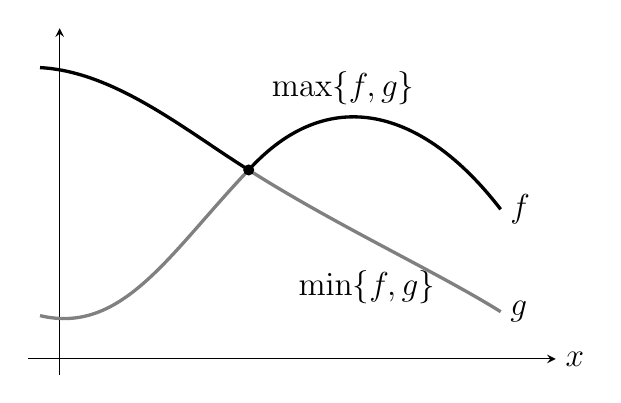
\begin{tikzpicture}[font=\large,>=stealth]
  \draw[->] (-0.4,0)--(6.3,0) node[right] {$x$};
  \draw[->] (0,-0.2)--(0,4.2);
  \draw[very thick,black!50]
    (-0.25,0.55)..controls (0.8,0.3) and (1.4,1.35)..(2.4,2.4);
  \draw[very thick]
    (2.4,2.4)..controls (3.4,3.5) and (4.6,3.2)..(5.6,1.9);
  \draw[very thick]
    (-0.25,3.7)..controls (0.7,3.65) and (1.6,2.9)..(2.4,2.4);
  \draw[very thick,black!50]
    (2.4,2.4)..controls (3.5,1.7) and (4.8,1.1)..(5.6,0.6);
  \fill (2.4,2.4) circle (2pt);
  \node[right] at (5.6,1.9) {$f$};
  \node[right] at (5.6,0.6) {$g$};
  \node[above] at (3.6,3.1) {$\max\{f,g\}$};
  \node[below] at (3.9,1.25) {$\min\{f,g\}$};
\end{tikzpicture}
\end{document}
